\subsection{The Capacitive Chair}
\begin{figure}[h]
\centering
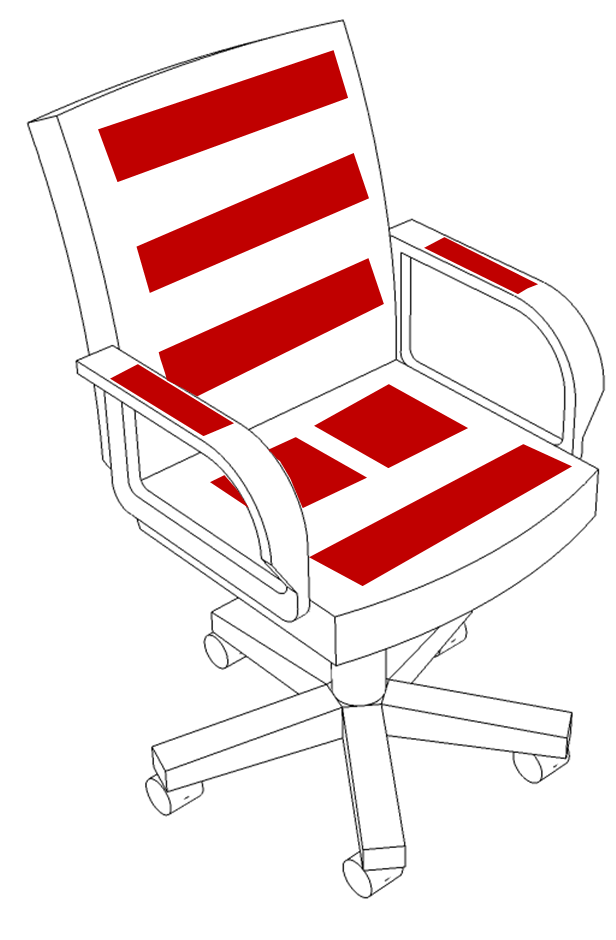
\includegraphics[width=0.4\textwidth]{images/smartofficechair}
\caption{Smart office chair sketch - eight electrodes three in backrest, three on seat and two in armrests}
\label{fig:smartchair_sketch}
\end{figure}
The Capacitive Chair is a regular office chair equipped with eight capacitive proximity sensors that can detect different sitting postures and work-related stress levels by examining movement and breathing rate \cite{Braun2013ChairAid}. Seven solid copper electrodes that are placed below the covering are augmented by a single conductive thread electrode that is placed in a mesh on the backrest. In the past smart chairs have used pressure sensors to infer posture and occupation \cite{tan2001sensing}. Combining presence and proximity sensing it is possible to directly infer postures where parts of the body do not touch the surface, e.g. if the body is arched towards the front, or if an arm is raised from the armrests. Additionally higher area electrodes in the backrest allow detecting the breathing rate by measuring the movement of the chest.

The Capacitive Chair aims at providing different services to a typical office worker and office managers. Using the occupation detection it is possible to advise for some type of physical activity, if the time spent in front of the screen was too long. The system can also advise the user to change to a more back-friendly posture or regularly switch the stance to achieve a more general workout. Using the breathing rate detection we are able to get some sort of measure of the current stress level associated to the given working situation. By adapting the environment it is possible to improve the working atmosphere and reduce stress. The Capacitive Chair uses a multifacetted data processing approach. A machine learning algorithm is associating the sensing data to one of nine different typical sitting positions, inspired by a recent study of sitting positions for modern device usage \cite{globalPosture}. An adaptive body model that is fitted to the current sensor values allows for fine grained adaptation of those postures. Finally a combination of Fourier and data variation analysis is calculating the current breathing rate \cite{Braun2013ChairAid}.

\subsubsection{Evaluation}
\begin{figure}[h]
\centering
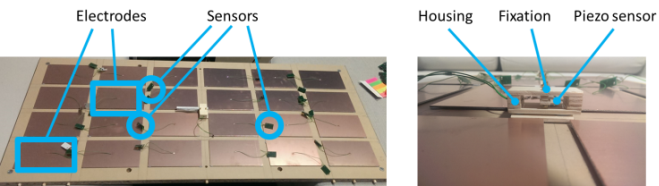
\includegraphics[width=0.7\textwidth]{images/captap_proto}
\caption{Detail views of the prototype system: left - electrode and sensors, right - knock detection box \cite{Braun2013ChairAid}}
\label{fig:captap_proto}
\end{figure}
%Figure 35 Detail views of the prototype system: left - electrode and sensors, right - knock detection box [80]
The CapTap prototype is integrated into a common living room table. Some photos can be seen in Figure \ref{fig:captap_proto}. On the left side we see the 24 electrodes made of non-etched circuit boards. A sensor is attached to each. The knock detection box with fixation, housing and piezo sensor is shown on the right side.
\begin{figure}[h]
\centering
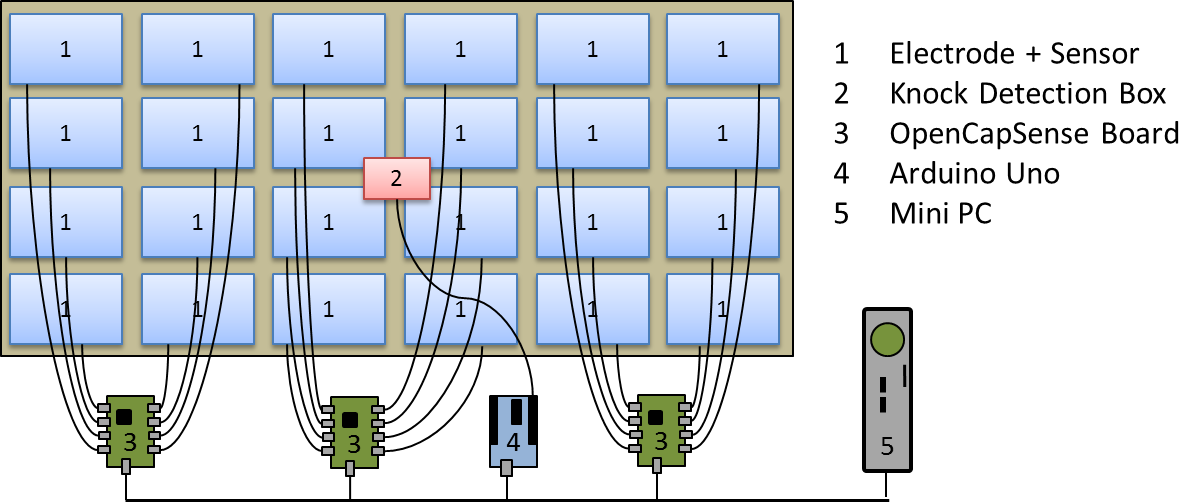
\includegraphics[width=0.7\textwidth]{images/captap_system}
\caption{Abstracted view of CapTap prototype including capacitive sensing electrodes and knock detection sensor \cite{Braun2013ChairAid}}
\label{fig:captap_system}
\end{figure} 
%Figure 36 Abstracted view of CapTap prototype including capacitive sensing electrodes and knock detection sensor [80]
The overall abstracted layout of the prototype is shown in Figure \ref{fig:captap_system}. The capacitive sensors are con-trolled by three OpenCapSense boards; the knock detection is performed on an Arduino Uno microcontroller board. The data fusion is outsourced to a Mini-PC that can be placed in the table.
Various evaluations have been performed with the CapTap. We have benchmarked the hand localization against the Leap Motion, concluding that the algorithm works reasonably precise in most parts of the interaction area. The next study was a quantitative study of the percentage of correctly recognized knocks, resulting in considerable misattribution of single and double knocks, due to strongly varying knocking styles. However, the presence of any knock was detected with a precision of about $90\%$ \cite{Braun2013ChairAid}. Our main evaluation of the system was concerned with the influence of our knock detection on the overall interaction speed of the system. The results concluded that merely adding the knock detection is not enough but that additionally the interfaces have to be adapted towards capacitive systems \cite{Braun2013ChairAid}.
